\problemname{Laser Strike}

Ann and her friend Kathrin have recently discovered a new board game that has become their favourite: Laser Strike.
In this game, the two players work together to remove $N$ pieces from the board.
The game runs in two phases.
The catch is that Kathrin will not have complete information about the game.
In order to win the game, Ann and Kathrin have to work together, while communicating as little as possible.

There are $N$ unique pieces on the board, numbered from $0$ to $N-1$. 
Both players can see these pieces.
There are also $N-1$ connections between pairs of pieces, such that it is possible to reach any piece from any other piece by following these connections.
In other words, these connections form a tree.
\textbf{Only Ann can see these connections; Kathrin does not know them.}

In the first phase of the game, Ann decides on an order $\ell_0, \ell_1, \ldots, \ell_{N-2}$ in which pieces should be removed, until there is only one left. 
This order will be kept secret from Kathrin. If she can replicate it, they will win the game.
The removal of pieces must satisfy the following rule: every time a piece is removed, it must be connected with exactly one remaining piece.
In other words, the removed piece must be a leaf of the tree formed by the remaining pieces and itself.
(After the $N-1$ pieces have been removed, the last piece is removed automatically and the players win.)
Ann must choose an order that corresponds to the above rule.

Ann will also write down a message to Kathrin, in the form of a binary string.
Ann can choose how long this message is -- but the shorter it is, the more points they get.

After that, the second phase of the game starts.
The goal of the game is for Kathrin to remove $N-1$ pieces from the board in the order $\ell_0, \ell_1, \ldots, \ell_{N-2}$.
She will make $N-1$ moves.
Before move $i$, Ann tells Kathrin a pair of integers $a$, $b$ with the following properties:

\begin{itemize}
\item $a < b$;
\item there is still a pair of directly connected pieces with numbers $a$ and $b$; and
\item either $a$ or $b$ is the correct piece $\ell_i$ that should be removed in this move.
\end{itemize}

Note that for Ann the connection $(a,b)$ is uniquely determined by the leaf $\ell_i$ in the current tree. 

Kathrin then removes either $a$ or $b$ from the board.
If this was the correct piece -- that is, $\ell_i$ -- they keep playing.
Otherwise they lose the game. 

Your task is to implement both Ann's and Kathrin's strategies so that they win the game.

Your program will be scored depending on the length of the message that Ann writes in the first phase of the game.

\section*{Implementation}
This is a multi-run problem, meaning that your program will be executed twice.
The first time it is run, it should implement Ann's strategy for the first phase of the game. 
After that, it should implement Kathrin's strategy for the second phase of the game.

The first line of the input contains two integers, $P$ and $N$, where $P$ is either $1$ or $2$ (first or second phase),
and $N$ is the number of pieces.

The following input depends on the phase:

\subsection*{\textbf{Phase 1}: Ann}

After the first line (described above) the next $N - 1$ lines of the input describe the tree.
Each line contains two numbers, $a$ and $b$ ($0 \le a < b \le N-1$), indicating a connection between pieces $a$ and $b$.

Your program should begin by outputting a binary string with at most $1\,000$ characters, each `\verb@0@' or `\verb@1@', the message written by Ann.
Note that to generate a string of length $0$, it should output an empty line.

After this, it should output $N - 1$ integers $\ell_0, \ell_1, \ldots, \ell_{N-2}$ on separate lines, indicating the order in which Ann wants to remove the leaves of the tree.
The order must be such that if the pieces are removed one by one from the tree in this order, the removed piece must always be a leaf, i.e., the tree must always remain connected.

\subsection*{\textbf{Phase 2}: Kathrin}


After the first line (described above), the next line of input contains the binary string (Ann's message) from Phase 1.

After this, there will be $N-1$ rounds of interaction, one for each of Kathrin's moves. 

In the $i$th move, 
your program should first read two numbers, $a$ and $b$  ($0\le a < b \le N-1$).
One of these pieces is the leaf $\ell_i$ in Ann's order, and the other piece is the only remaining piece connected to $\ell_i$. 
Then, your program should output $\ell_i$, indicating that Kathrin removes this leaf. If your program does not print the correct leaf $\ell_i$, the girls lose the game and your submission will be judged as Wrong Answer for this test case.


\paragraph{Details.}
If the \textit{sum} of the running times of the two separate runs of your program exceeds the time limit, your submission will be judged as Time Limit Exceeded.

Make sure to flush standard output after printing each line, or else your program might be judged as Time Limit Exceeded.
In Python, this happens automatically as long as you use \texttt{input()} to read lines. In C++, \texttt{cout << endl;} flushes in addition to printing a newline; if using printf, use \texttt{fflush(stdout);}.

Note that correctly reading an empty string can be tricky. The provided templates handle this case correctly.

\section*{Constraints and Scoring}
\begin{itemize}
    \item $N = 1\,000$.
    \item $0 \le a < b \le N-1$ for all connections.
\end{itemize}

Your solution will be tested on a set of test groups, each worth a number of points.
Each test group contains a set of test cases. To get the points for a test group, you need to
solve all test cases in the test group.

\begin{tabular}{|l|l|l|}
\hline
Group  &  Max score  &  Constraints \\
\hline
 1 & 8 & The tree is a star. That is, all nodes except one are leaves.   \\
\hline
 2 & 9 & The tree is a line. That is, all nodes except for two leaf nodes have exactly two adjacent nodes.  \\
\hline
 3 & 21 & The tree is a star with lines going out from it. That is, all nodes have either one or two adjacent nodes, except for one that has more than two adjacent nodes.   \\
\hline
 4 & 36 & The distance between any two nodes is at most $10$.   \\
\hline
 5 & 26 & No additional constraints.  \\
\hline
\end{tabular}

For every test group that your program solves correctly, you will receive a score based on the following formula:
\[\text{score} = S_g \cdot \left(1 - 0.3 \cdot \log_{10} \max(K, 1) \right),\]
where $S_g$ is the maximum score for the test group,
and $K$ is the maximum length of Ann's message needed
for any test case in the test group.
\textbf{Your score for each test group will be rounded to the nearest integer.}

The table below shows the number of points, for a few values of $K$, that your program will get if it solves all test groups with that $K$.
In particular, to achieve a score of $100$ points, your solution must solve every test case with $K\le 1$. 

\begin{tabular}{|c|c|c|c|c|c|c|c|}
    \hline
    \textbf{K}  &  1  &  5 & 10 & 50 & 100 & 500 & 1000  \\
    \hline
    \textbf{Score} & 100 & 79 & 70 & 49 & 39 & 20 & 11   \\
    \hline
\end{tabular}

\section*{Testing Tool}
To facilitate the testing of your solution, we have provided a simple tool that you can download.
See `attachments' at the bottom of the Kattis problem page.
The tool is optional to use. Note that the official grader program on Kattis is different from the testing tool.

To use the tool, create an input file, such as `sample1.in', which should start with a number $N$ followed by $N-1$ lines describing the tree, in the same format as in Phase 1.
For example, for the sample below:

\begin{verbatim}
7
0 1
1 2
2 3
0 4
0 6
1 5
\end{verbatim}

For Python programs, say \texttt{solution.py} (normally run as \texttt{pypy3 solution.py}):

    \verb|python3 testing_tool.py pypy3 solution.py < sample1.in|

For C++ programs, first compile it
(e.g. with \texttt{g++ -g -O2 -std=gnu++23 -static solution.cpp -o solution.out})
and then run:

    \verb|python3 testing_tool.py ./solution.out < sample1.in|

\section*{Example}
Note that the sample in this section has $N = 7$ for simplicity and is therefore not a valid test case. Your program is not expected to be able to solve this case. All test cases on the grader will have $N = 1\,000$.

In the sample, Ann is given the following tree. In the first phase, Ann reads the tree, selects a binary string "\verb|0110|" to send to Kathrin, and also selects an order $[\ell_0, \ell_1, \ldots \ell_{N-2}] = [5,3,2,6,4,0]$ in which the pieces should be removed from the tree.
In the second phase, Kathrin receives the string "\verb|0110|" that was sent in the first phase. 
She then receives the pair $(1, 5)$ and decides to remove vertex $5$, which is indeed the leaf. 
For the next move, she receives the pair $(2, 3)$ and removes the leaf $3$, and so on.
The following pictures depict the interactions:

\begin{figure}
\centering
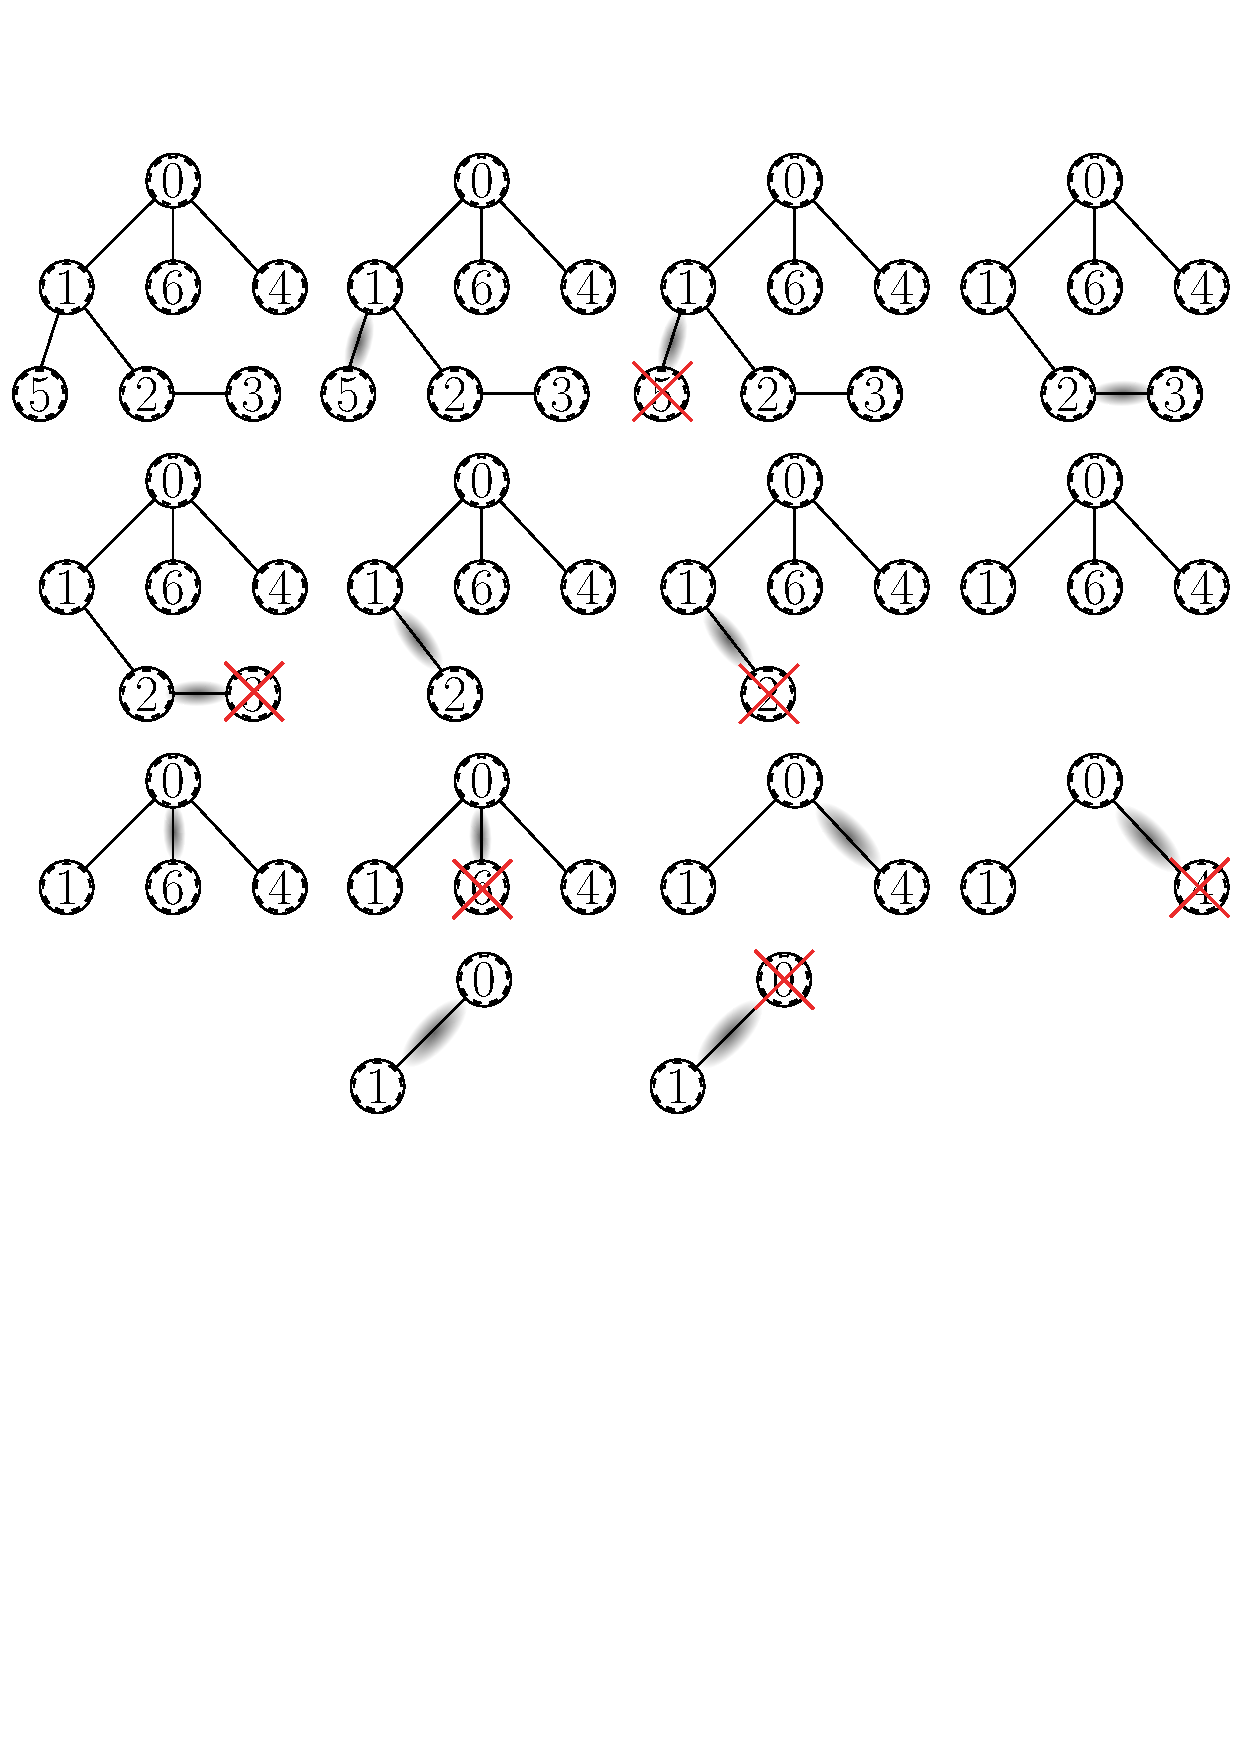
\includegraphics[width=0.95\textwidth]{sample_interaction}
\end{figure}


